% Auto-generated by r_project/results/step5_diagnostics.R at commit 8585b0d (uncommitted changes)

\begin{figure}[htbp]
\centering
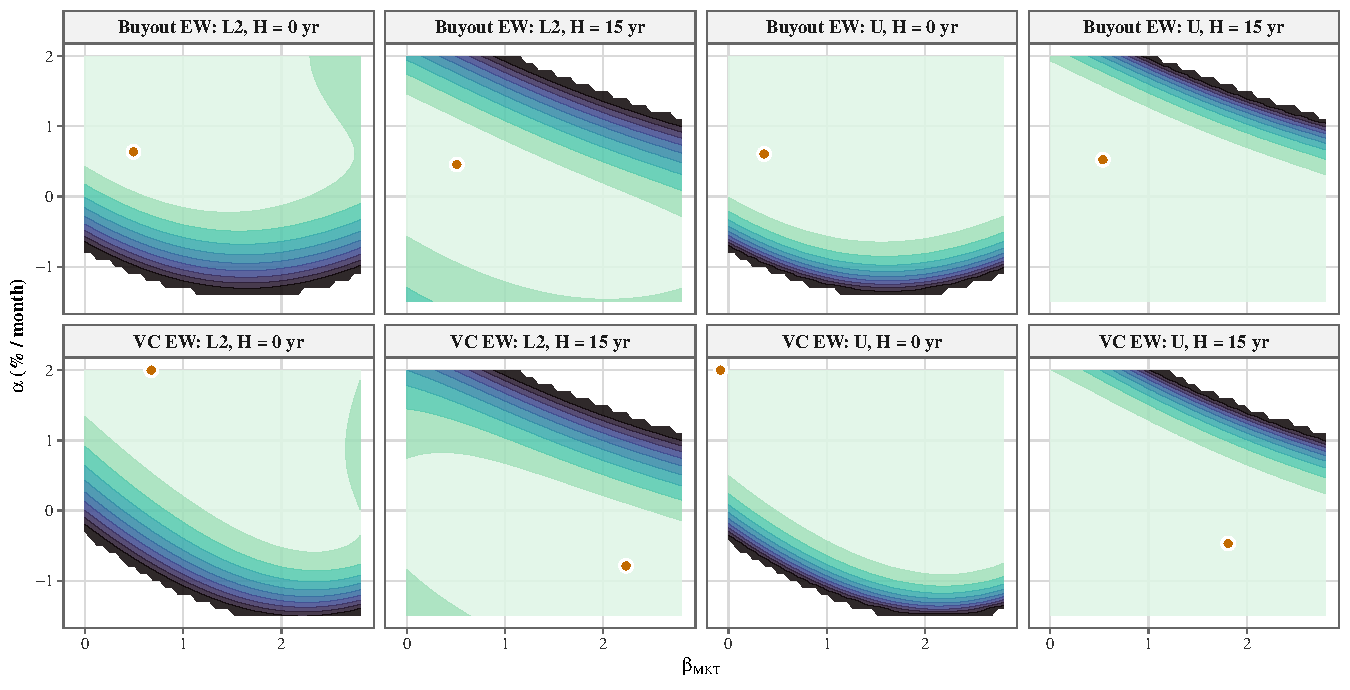
\includegraphics[width=\textwidth]{figure_S5_alpha_beta_contours.pdf}
\caption{Normalized $(\alpha,\beta)$ criterion contours for Buyout and Venture Capital (EW) at $H=0$ and $H=15$ years}
\label{fig:alpha_beta_contours}
\par\vspace{2pt}
{\scriptsize\textit{Notes:} Normalized criterion surfaces $(Q(\alpha,\beta)-Q_{\min})/(Q_{0.90}-Q_{\min})$ over $\beta\in[0,2.8]$ and $\alpha\in[-1.5\%,2\%]$ per month (darker shading = lower criterion; orange circle = constrained optimum on $\Theta$). Top/bottom rows compare Buyout EW (well-defined negatively sloped interior valley reflecting the negative $(\hat\alpha,\hat\beta)$ trade-off) with VC EW (at $H=0$ the surface falls monotonically to the $+2\%$ monthly $\alpha$ upper bound under both L2 and $U_{v,H}$, whereas $H=15$ imposes coercivity without identifying $\alpha$).}
\end{figure}
